\section{Messwerte und Auswertung} % (fold)
\label{sec:messwerte_und_auswertung}

	\subsection{Temperaturverteilung} % (fold)
	\label{sub:temperaturverteilung}
	
		Um eine Vorstellung des genauen Temperaturverlaufs innerhalb der Kühlkanne zu bekommen, wurde die Temperatur an einigen markanten Stellen über Widerstandsmessung des Pt1000 Drahts sowie über die Diode bestimmt.
		Wie erwartet lief der metallische Widerstand auf einen konstanten Restwiderstand hinaus.
		Dadurch konnte die Temperatur unterhalb von $20\unit{K}$ nur noch sehr unzuverlässig bestimmt werden.


	% subsection temperaturverteilung (end)


	% \subsection{Beurteilung der Farbe der Kühlkanne} % (fold)
	% \label{sub:beurteilung_der_farbe_der_k_hlkanne}
	% 	Die Farbe der Kühlkanne ließ sich nur schwer mit den uns zur Verfügung stehenden Mitteln bestimmen. Sicher feststellen konnten wir allerdings, dass die Farbe hervoragend in die karge und abstoßende Atmosphäre des Raumes 
	% 	passt. 

	% % subsection beurteilung_der_farbe_der_k_hlkanne (end)


	\subsection{Supraleitung von Tantal} % (fold)
	\label{sub:supraleitung_von_tantal}

		Mit Hilfe der Werte aus Abschnitt \ref{sub:temperaturverteilung} konnte nun ein Tantal-Draht an die richtige Position und Temperatur gebracht werden, dass der Effekt der Supraleitung gezeigt wurde.
		Abbildung \ref{widerstandsabfall} zeigt eindeutig den schlagartigen Abfall des Restwiderstands bei einem gewissen Widerstandswert der Diode.
		\begin{figure}
			% \center
			% GNUPLOT: LaTeX picture with Postscript
\begingroup
  \makeatletter
  \providecommand\color[2][]{%
    \GenericError{(gnuplot) \space\space\space\@spaces}{%
      Package color not loaded in conjunction with
      terminal option `colourtext'%
    }{See the gnuplot documentation for explanation.%
    }{Either use 'blacktext' in gnuplot or load the package
      color.sty in LaTeX.}%
    \renewcommand\color[2][]{}%
  }%
  \providecommand\includegraphics[2][]{%
    \GenericError{(gnuplot) \space\space\space\@spaces}{%
      Package graphicx or graphics not loaded%
    }{See the gnuplot documentation for explanation.%
    }{The gnuplot epslatex terminal needs graphicx.sty or graphics.sty.}%
    \renewcommand\includegraphics[2][]{}%
  }%
  \providecommand\rotatebox[2]{#2}%
  \@ifundefined{ifGPcolor}{%
    \newif\ifGPcolor
    \GPcolorfalse
  }{}%
  \@ifundefined{ifGPblacktext}{%
    \newif\ifGPblacktext
    \GPblacktexttrue
  }{}%
  % define a \g@addto@macro without @ in the name:
  \let\gplgaddtomacro\g@addto@macro
  % define empty templates for all commands taking text:
  \gdef\gplbacktext{}%
  \gdef\gplfronttext{}%
  \makeatother
  \ifGPblacktext
    % no textcolor at all
    \def\colorrgb#1{}%
    \def\colorgray#1{}%
  \else
    % gray or color?
    \ifGPcolor
      \def\colorrgb#1{\color[rgb]{#1}}%
      \def\colorgray#1{\color[gray]{#1}}%
      \expandafter\def\csname LTw\endcsname{\color{white}}%
      \expandafter\def\csname LTb\endcsname{\color{black}}%
      \expandafter\def\csname LTa\endcsname{\color{black}}%
      \expandafter\def\csname LT0\endcsname{\color[rgb]{1,0,0}}%
      \expandafter\def\csname LT1\endcsname{\color[rgb]{0,1,0}}%
      \expandafter\def\csname LT2\endcsname{\color[rgb]{0,0,1}}%
      \expandafter\def\csname LT3\endcsname{\color[rgb]{1,0,1}}%
      \expandafter\def\csname LT4\endcsname{\color[rgb]{0,1,1}}%
      \expandafter\def\csname LT5\endcsname{\color[rgb]{1,1,0}}%
      \expandafter\def\csname LT6\endcsname{\color[rgb]{0,0,0}}%
      \expandafter\def\csname LT7\endcsname{\color[rgb]{1,0.3,0}}%
      \expandafter\def\csname LT8\endcsname{\color[rgb]{0.5,0.5,0.5}}%
    \else
      % gray
      \def\colorrgb#1{\color{black}}%
      \def\colorgray#1{\color[gray]{#1}}%
      \expandafter\def\csname LTw\endcsname{\color{white}}%
      \expandafter\def\csname LTb\endcsname{\color{black}}%
      \expandafter\def\csname LTa\endcsname{\color{black}}%
      \expandafter\def\csname LT0\endcsname{\color{black}}%
      \expandafter\def\csname LT1\endcsname{\color{black}}%
      \expandafter\def\csname LT2\endcsname{\color{black}}%
      \expandafter\def\csname LT3\endcsname{\color{black}}%
      \expandafter\def\csname LT4\endcsname{\color{black}}%
      \expandafter\def\csname LT5\endcsname{\color{black}}%
      \expandafter\def\csname LT6\endcsname{\color{black}}%
      \expandafter\def\csname LT7\endcsname{\color{black}}%
      \expandafter\def\csname LT8\endcsname{\color{black}}%
    \fi
  \fi
  \setlength{\unitlength}{0.0500bp}%
  \begin{picture}(6802.00,3826.00)%
    \gplgaddtomacro\gplbacktext{%
      \csname LTb\endcsname%
      \put(946,704){\makebox(0,0)[r]{\strut{}0.10}}%
      \put(946,1275){\makebox(0,0)[r]{\strut{}0.15}}%
      \put(946,1847){\makebox(0,0)[r]{\strut{}0.20}}%
      \put(946,2418){\makebox(0,0)[r]{\strut{}0.25}}%
      \put(946,2990){\makebox(0,0)[r]{\strut{}0.30}}%
      \put(946,3561){\makebox(0,0)[r]{\strut{}0.35}}%
      \put(1078,484){\makebox(0,0){\strut{}-0.1}}%
      \put(1966,484){\makebox(0,0){\strut{}0.0}}%
      \put(2854,484){\makebox(0,0){\strut{}0.1}}%
      \put(3742,484){\makebox(0,0){\strut{}0.2}}%
      \put(4629,484){\makebox(0,0){\strut{}0.3}}%
      \put(5517,484){\makebox(0,0){\strut{}0.4}}%
      \put(6405,484){\makebox(0,0){\strut{}0.5}}%
      \put(176,2132){\rotatebox{-270}{\makebox(0,0){\strut{}$\textit{Spannung am Tantaldraht}$}}}%
      \put(3741,154){\makebox(0,0){\strut{}$\sim \textit{Spannung an Diode}$}}%
    }%
    \gplgaddtomacro\gplfronttext{%
      \csname LTb\endcsname%
      \put(5418,1427){\makebox(0,0)[r]{\strut{}Messwerte}}%
      \csname LTb\endcsname%
      \put(5418,1207){\makebox(0,0)[r]{\strut{}approximierter Kurvenverlauf}}%
    }%
    \gplbacktext
    \put(0,0){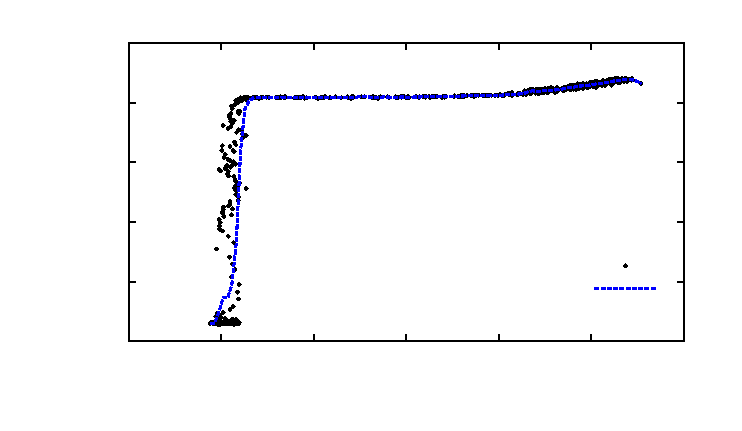
\includegraphics{gut}}%
    \gplfronttext
  \end{picture}%
\endgroup

			\caption{Spannungsverlauf des Tantal-Drahtes in Abhängigkeit der Temperatur (dargestellt durch Diodenspannung bei konstantem Diodenstrom von $10\unit{$\mu$A}$) \\ (aufgezeichnet durch LabView) }
			\label{widerstandsabfall}
		\end{figure}
		Die Diodenspannung wurde invertiert und mit einem Offset versehen, um den qualitativen Temperaturverlauf besser darzustellen.
		\par
		Im Folgenden wurde die Abhängigkeit der Sprungtemperatur vom äußeren Magnetfeld untersucht.
		Wie in Abbildung \ref{gap} zu sehen, stieg der Widerstand am Tantal-Draht je nach ein- oder ausgeschalteten Magnetfeld sprunghaft um $0.15\unit{V}$ an.
		Dies deutet auf eine Überschreitung der durch das Magnetfeld verringerten Sprungtemperatur hin.
		\begin{figure}
			% \center
			% GNUPLOT: LaTeX picture with Postscript
\begingroup
  \makeatletter
  \providecommand\color[2][]{%
    \GenericError{(gnuplot) \space\space\space\@spaces}{%
      Package color not loaded in conjunction with
      terminal option `colourtext'%
    }{See the gnuplot documentation for explanation.%
    }{Either use 'blacktext' in gnuplot or load the package
      color.sty in LaTeX.}%
    \renewcommand\color[2][]{}%
  }%
  \providecommand\includegraphics[2][]{%
    \GenericError{(gnuplot) \space\space\space\@spaces}{%
      Package graphicx or graphics not loaded%
    }{See the gnuplot documentation for explanation.%
    }{The gnuplot epslatex terminal needs graphicx.sty or graphics.sty.}%
    \renewcommand\includegraphics[2][]{}%
  }%
  \providecommand\rotatebox[2]{#2}%
  \@ifundefined{ifGPcolor}{%
    \newif\ifGPcolor
    \GPcolorfalse
  }{}%
  \@ifundefined{ifGPblacktext}{%
    \newif\ifGPblacktext
    \GPblacktexttrue
  }{}%
  % define a \g@addto@macro without @ in the name:
  \let\gplgaddtomacro\g@addto@macro
  % define empty templates for all commands taking text:
  \gdef\gplbacktext{}%
  \gdef\gplfronttext{}%
  \makeatother
  \ifGPblacktext
    % no textcolor at all
    \def\colorrgb#1{}%
    \def\colorgray#1{}%
  \else
    % gray or color?
    \ifGPcolor
      \def\colorrgb#1{\color[rgb]{#1}}%
      \def\colorgray#1{\color[gray]{#1}}%
      \expandafter\def\csname LTw\endcsname{\color{white}}%
      \expandafter\def\csname LTb\endcsname{\color{black}}%
      \expandafter\def\csname LTa\endcsname{\color{black}}%
      \expandafter\def\csname LT0\endcsname{\color[rgb]{1,0,0}}%
      \expandafter\def\csname LT1\endcsname{\color[rgb]{0,1,0}}%
      \expandafter\def\csname LT2\endcsname{\color[rgb]{0,0,1}}%
      \expandafter\def\csname LT3\endcsname{\color[rgb]{1,0,1}}%
      \expandafter\def\csname LT4\endcsname{\color[rgb]{0,1,1}}%
      \expandafter\def\csname LT5\endcsname{\color[rgb]{1,1,0}}%
      \expandafter\def\csname LT6\endcsname{\color[rgb]{0,0,0}}%
      \expandafter\def\csname LT7\endcsname{\color[rgb]{1,0.3,0}}%
      \expandafter\def\csname LT8\endcsname{\color[rgb]{0.5,0.5,0.5}}%
    \else
      % gray
      \def\colorrgb#1{\color{black}}%
      \def\colorgray#1{\color[gray]{#1}}%
      \expandafter\def\csname LTw\endcsname{\color{white}}%
      \expandafter\def\csname LTb\endcsname{\color{black}}%
      \expandafter\def\csname LTa\endcsname{\color{black}}%
      \expandafter\def\csname LT0\endcsname{\color{black}}%
      \expandafter\def\csname LT1\endcsname{\color{black}}%
      \expandafter\def\csname LT2\endcsname{\color{black}}%
      \expandafter\def\csname LT3\endcsname{\color{black}}%
      \expandafter\def\csname LT4\endcsname{\color{black}}%
      \expandafter\def\csname LT5\endcsname{\color{black}}%
      \expandafter\def\csname LT6\endcsname{\color{black}}%
      \expandafter\def\csname LT7\endcsname{\color{black}}%
      \expandafter\def\csname LT8\endcsname{\color{black}}%
    \fi
  \fi
  \setlength{\unitlength}{0.0500bp}%
  \begin{picture}(6802.00,3826.00)%
    \gplgaddtomacro\gplbacktext{%
      \csname LTb\endcsname%
      \put(946,1133){\makebox(0,0)[r]{\strut{}0.35}}%
      \put(946,1847){\makebox(0,0)[r]{\strut{}0.40}}%
      \put(946,2561){\makebox(0,0)[r]{\strut{}0.45}}%
      \put(946,3275){\makebox(0,0)[r]{\strut{}0.50}}%
      \put(1078,484){\makebox(0,0){\strut{}-0.02}}%
      \put(2410,484){\makebox(0,0){\strut{}-0.01}}%
      \put(3742,484){\makebox(0,0){\strut{}0.00}}%
      \put(5073,484){\makebox(0,0){\strut{}0.01}}%
      \put(6405,484){\makebox(0,0){\strut{}0.02}}%
      \put(176,2132){\rotatebox{-270}{\makebox(0,0){\strut{}$\textit{Spannung am Tantaldraht}$}}}%
      \put(3741,154){\makebox(0,0){\strut{}$\sim \textit{Spannung an Diode}$}}%
    }%
    \gplgaddtomacro\gplfronttext{%
      \csname LTb\endcsname%
      \put(5418,3388){\makebox(0,0)[r]{\strut{}Messwerte}}%
    }%
    \gplbacktext
    \put(0,0){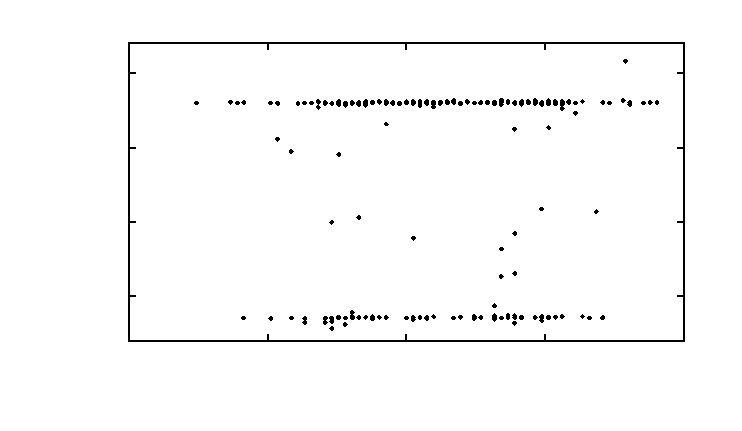
\includegraphics{gap2}}%
    \gplfronttext
  \end{picture}%
\endgroup

			\caption{Spannung des Tantal-Drahtes für ein- und ausgeschaltetes $B$-Feld. \\ (aufgezeichnet durch LabView)}
			\label{gap}
		\end{figure}

	% subsection supraleitung_von_tantal (end)


	\subsection{Gleichstrom Josephson-Kontakt} % (fold)
	\label{sub:gleichstrom_josephson_kontakt}
	
		Der SIS-Kontakt wurde wie in Abschnitt \ref{sec:aufbau_und_durchf_hrung} beschrieben hergestellt.
		Der rein supraleitende Fall ist in Abbildung \ref{waag_strich} zu sehen. 
		Wie erwartet fällt keine Spannung über dem Kontakt ab, da die Cooper-Paare widerstandslos durch die Leiter gehen und über die Isolatorschicht tunneln.
		\begin{figure}
			\center
			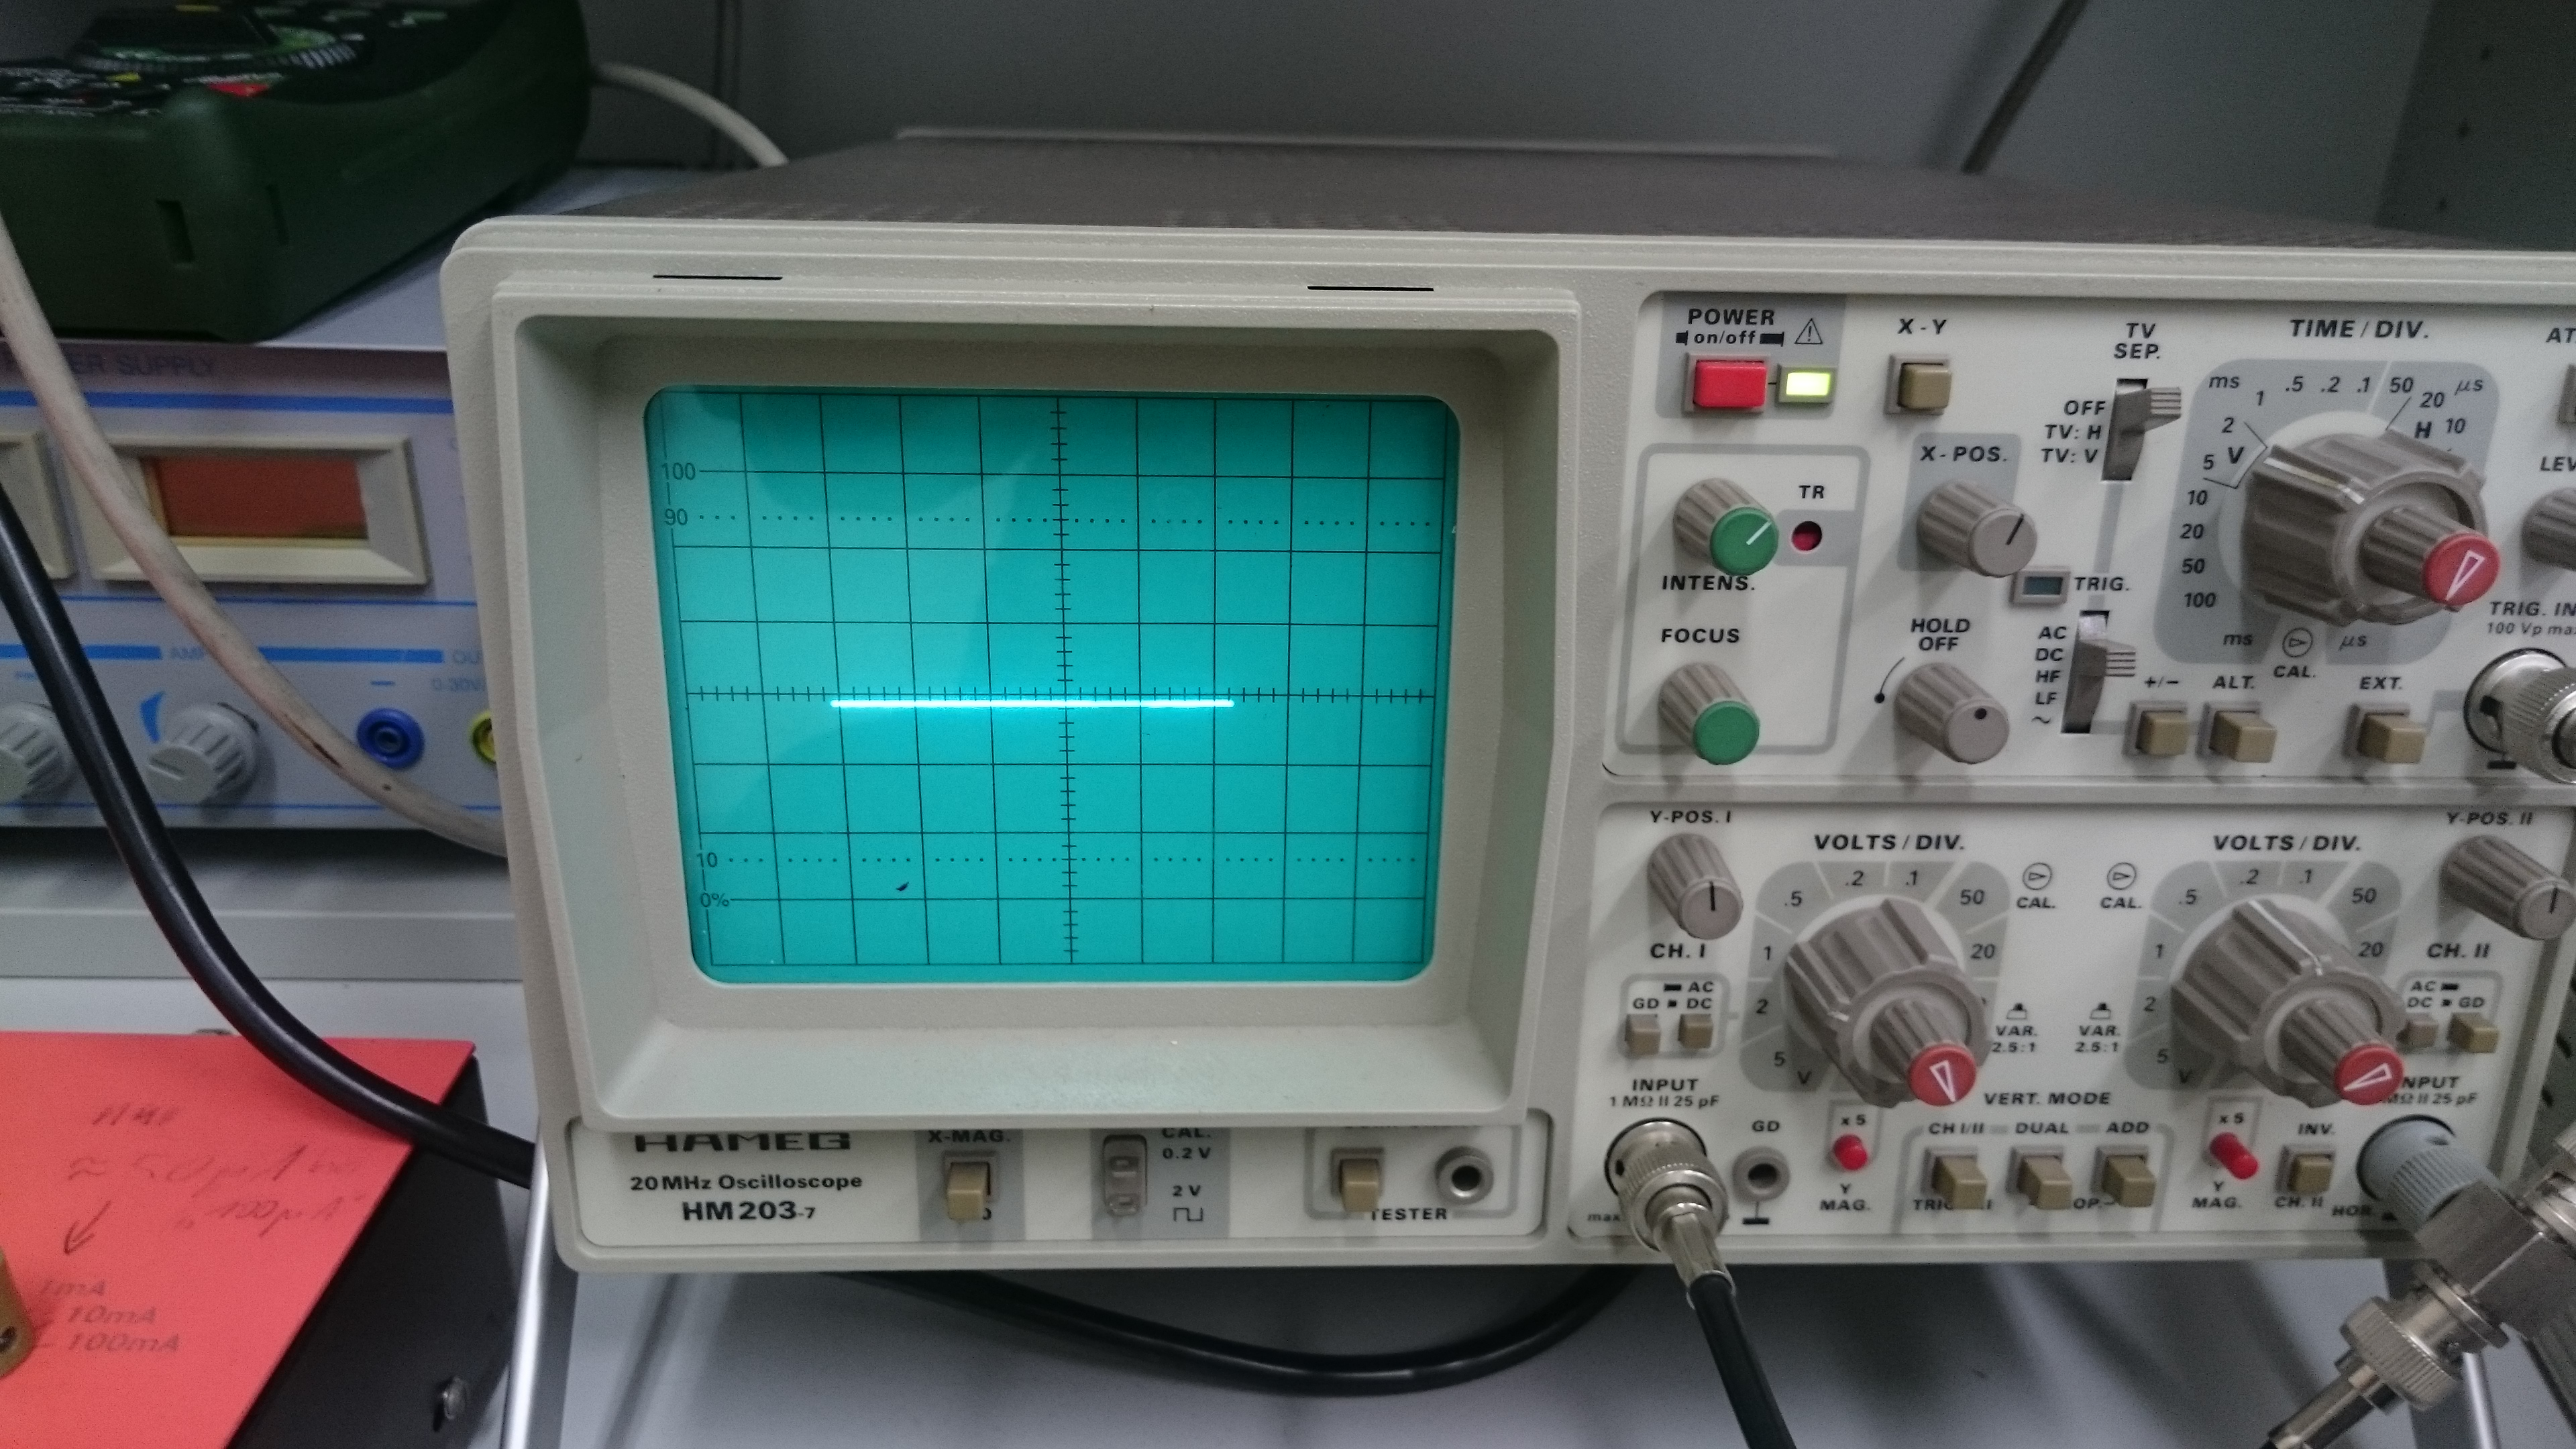
\includegraphics[scale=0.08]{messwerte/DSC_0618.JPG}
			\caption{Tantalspannung über Strom am Oszilloskop}
			\label{waag_strich}
		\end{figure}
		Bei größerem Wechselstrom konnte das vorhergesagte Verhalten mit Wechsel zwischen ohmschem und supraleitendem Zustand (siehe Abbildung \ref{zickzack}) beobachtet werden.
		\begin{figure}
			\center
			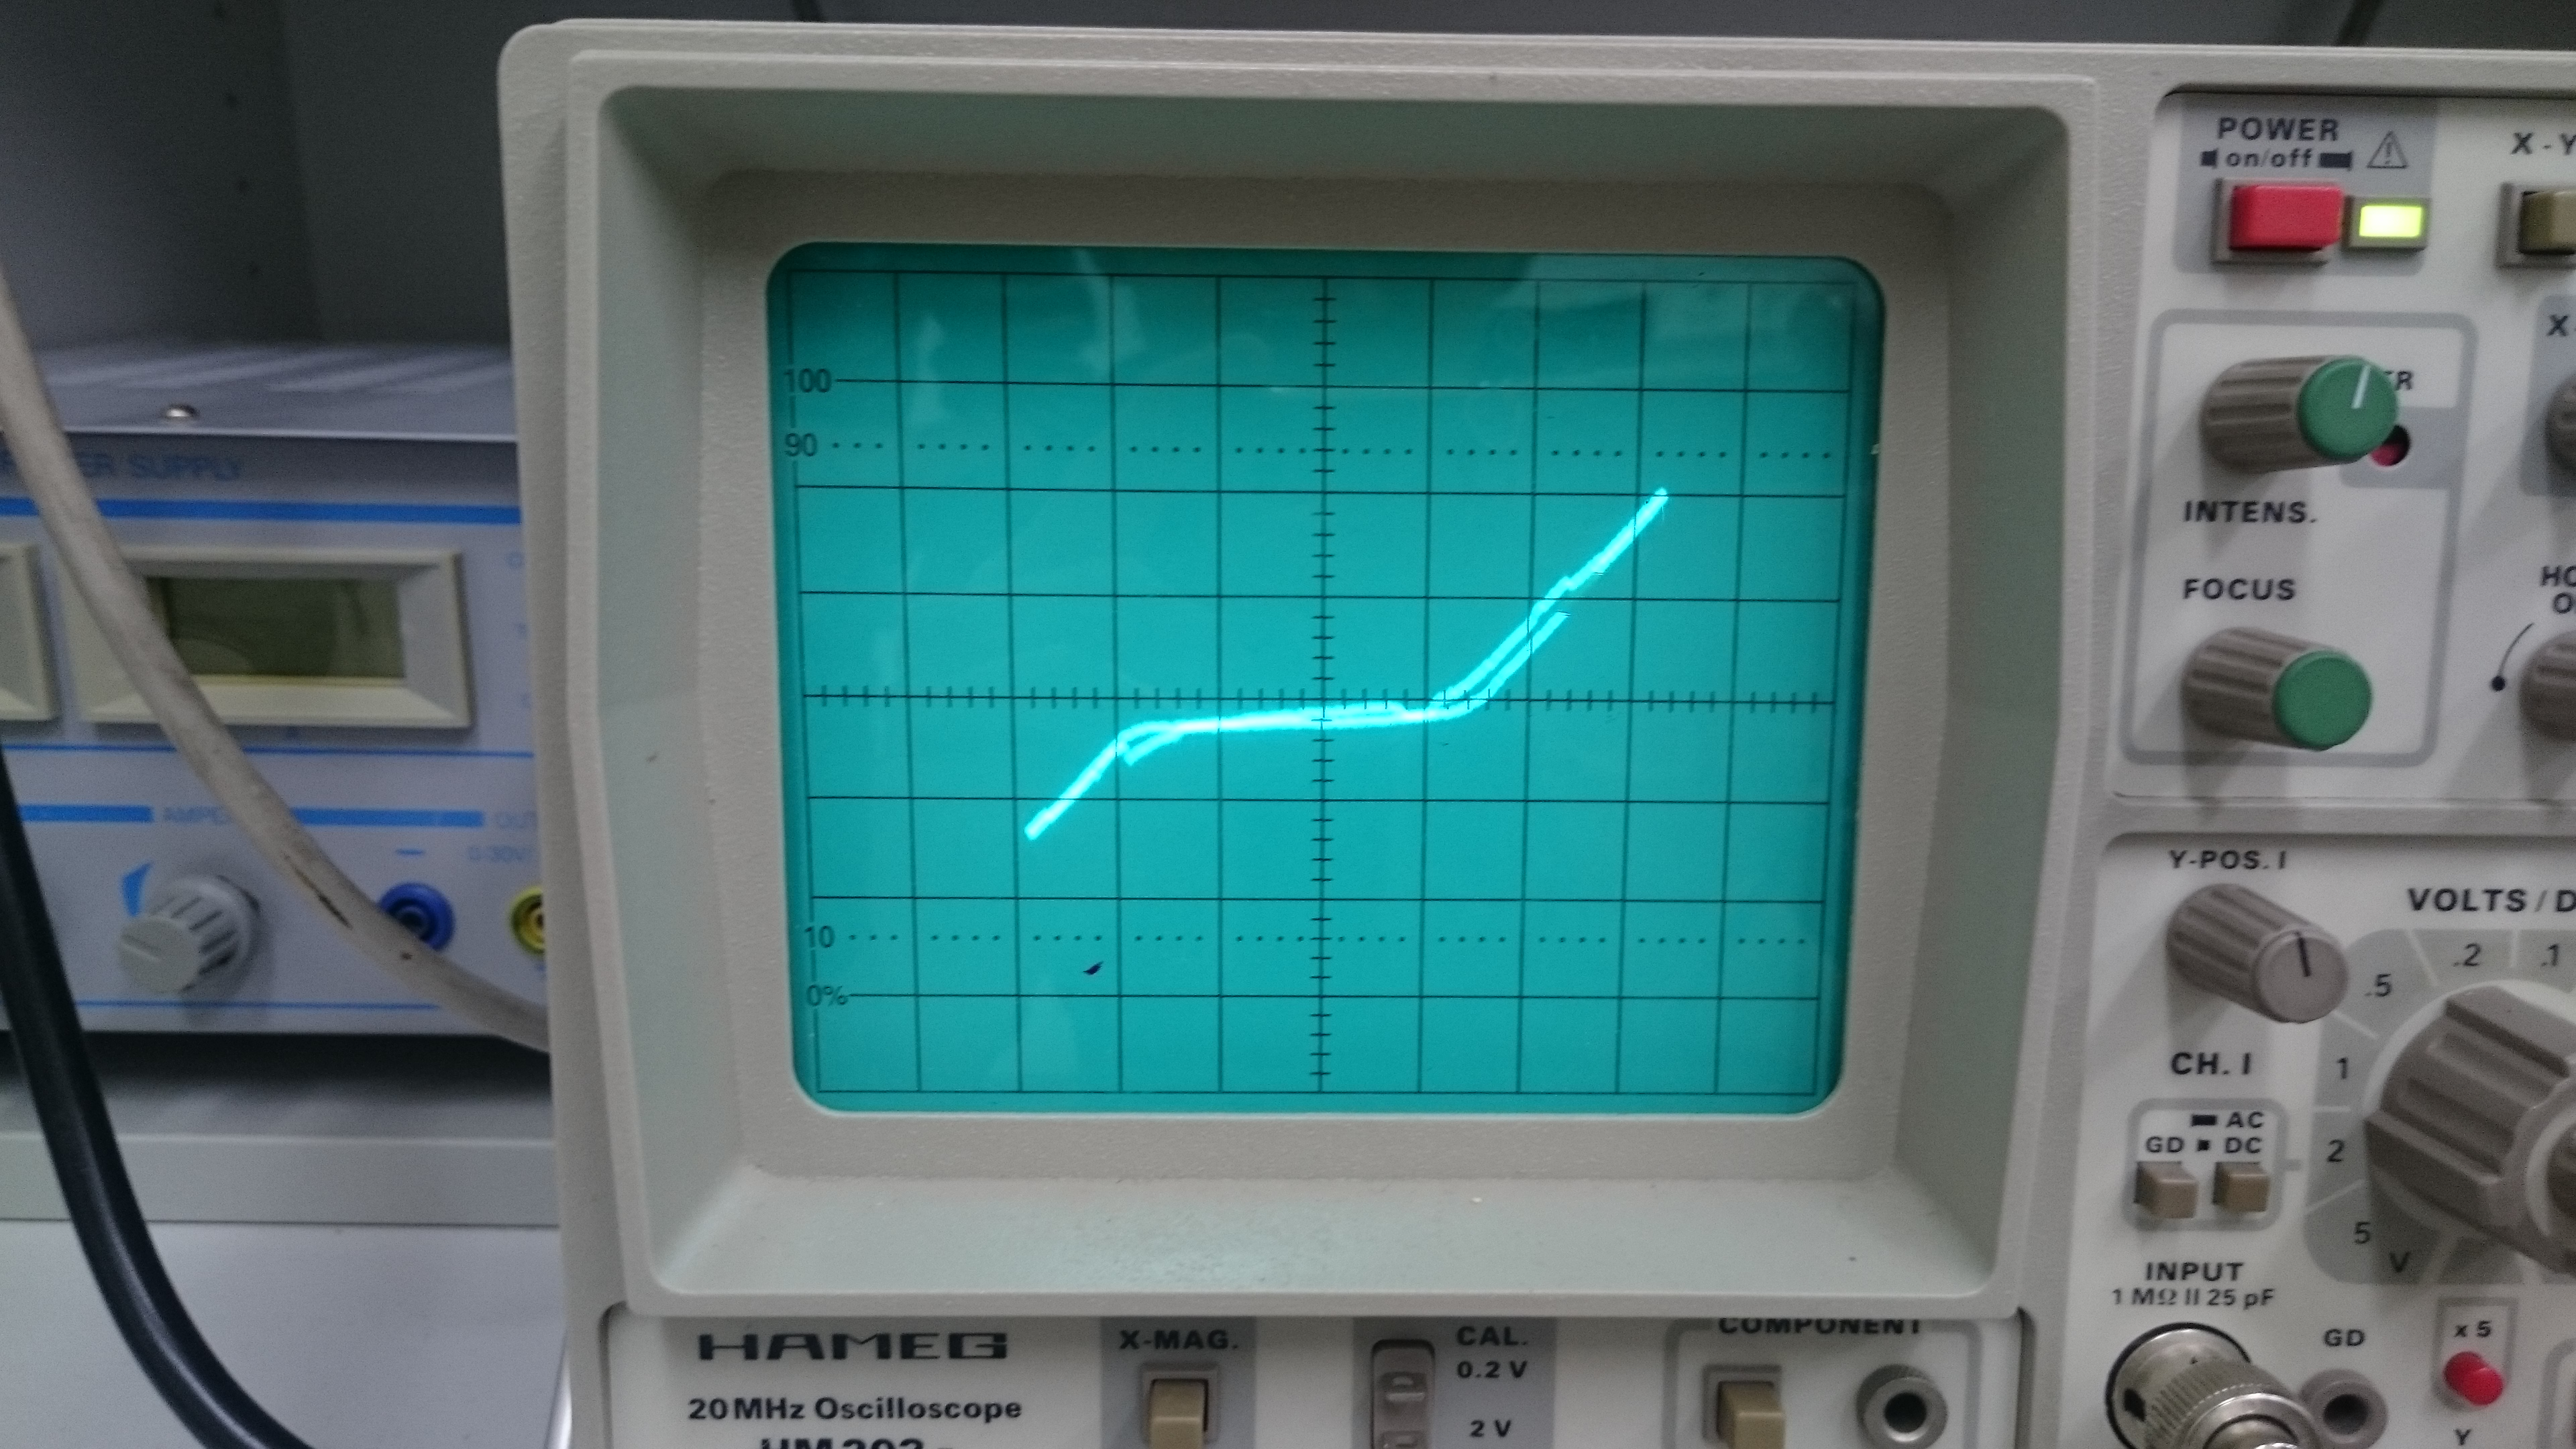
\includegraphics[scale=0.08]{messwerte/DSC_0624.JPG}
			\caption{Tantalspannung über Strom am Oszilloskop bei größerem Betrag des Wechselstromes}
			\label{zickzack}
		\end{figure}
		Oberhalb des positiven und unterhalb des negativen kritischen Stromes fällt wieder eine Spannung proportional zur durchfließenden Stromstärke ab.
		Durch Einkoppeln des Mikrowellenstrahlers wurde zwar eine Annäherung an die erwartete monoton steigende gewellte Gerade erreicht, allerdings reichte der Effekt nicht aus, um eindeutige Stufen wie in der Theorie prognostiziert zu sehen. 
		Ein Beispielbild ist in Abbildung \ref{nichtwelle} zu sehen:
		\begin{figure}
			\center
			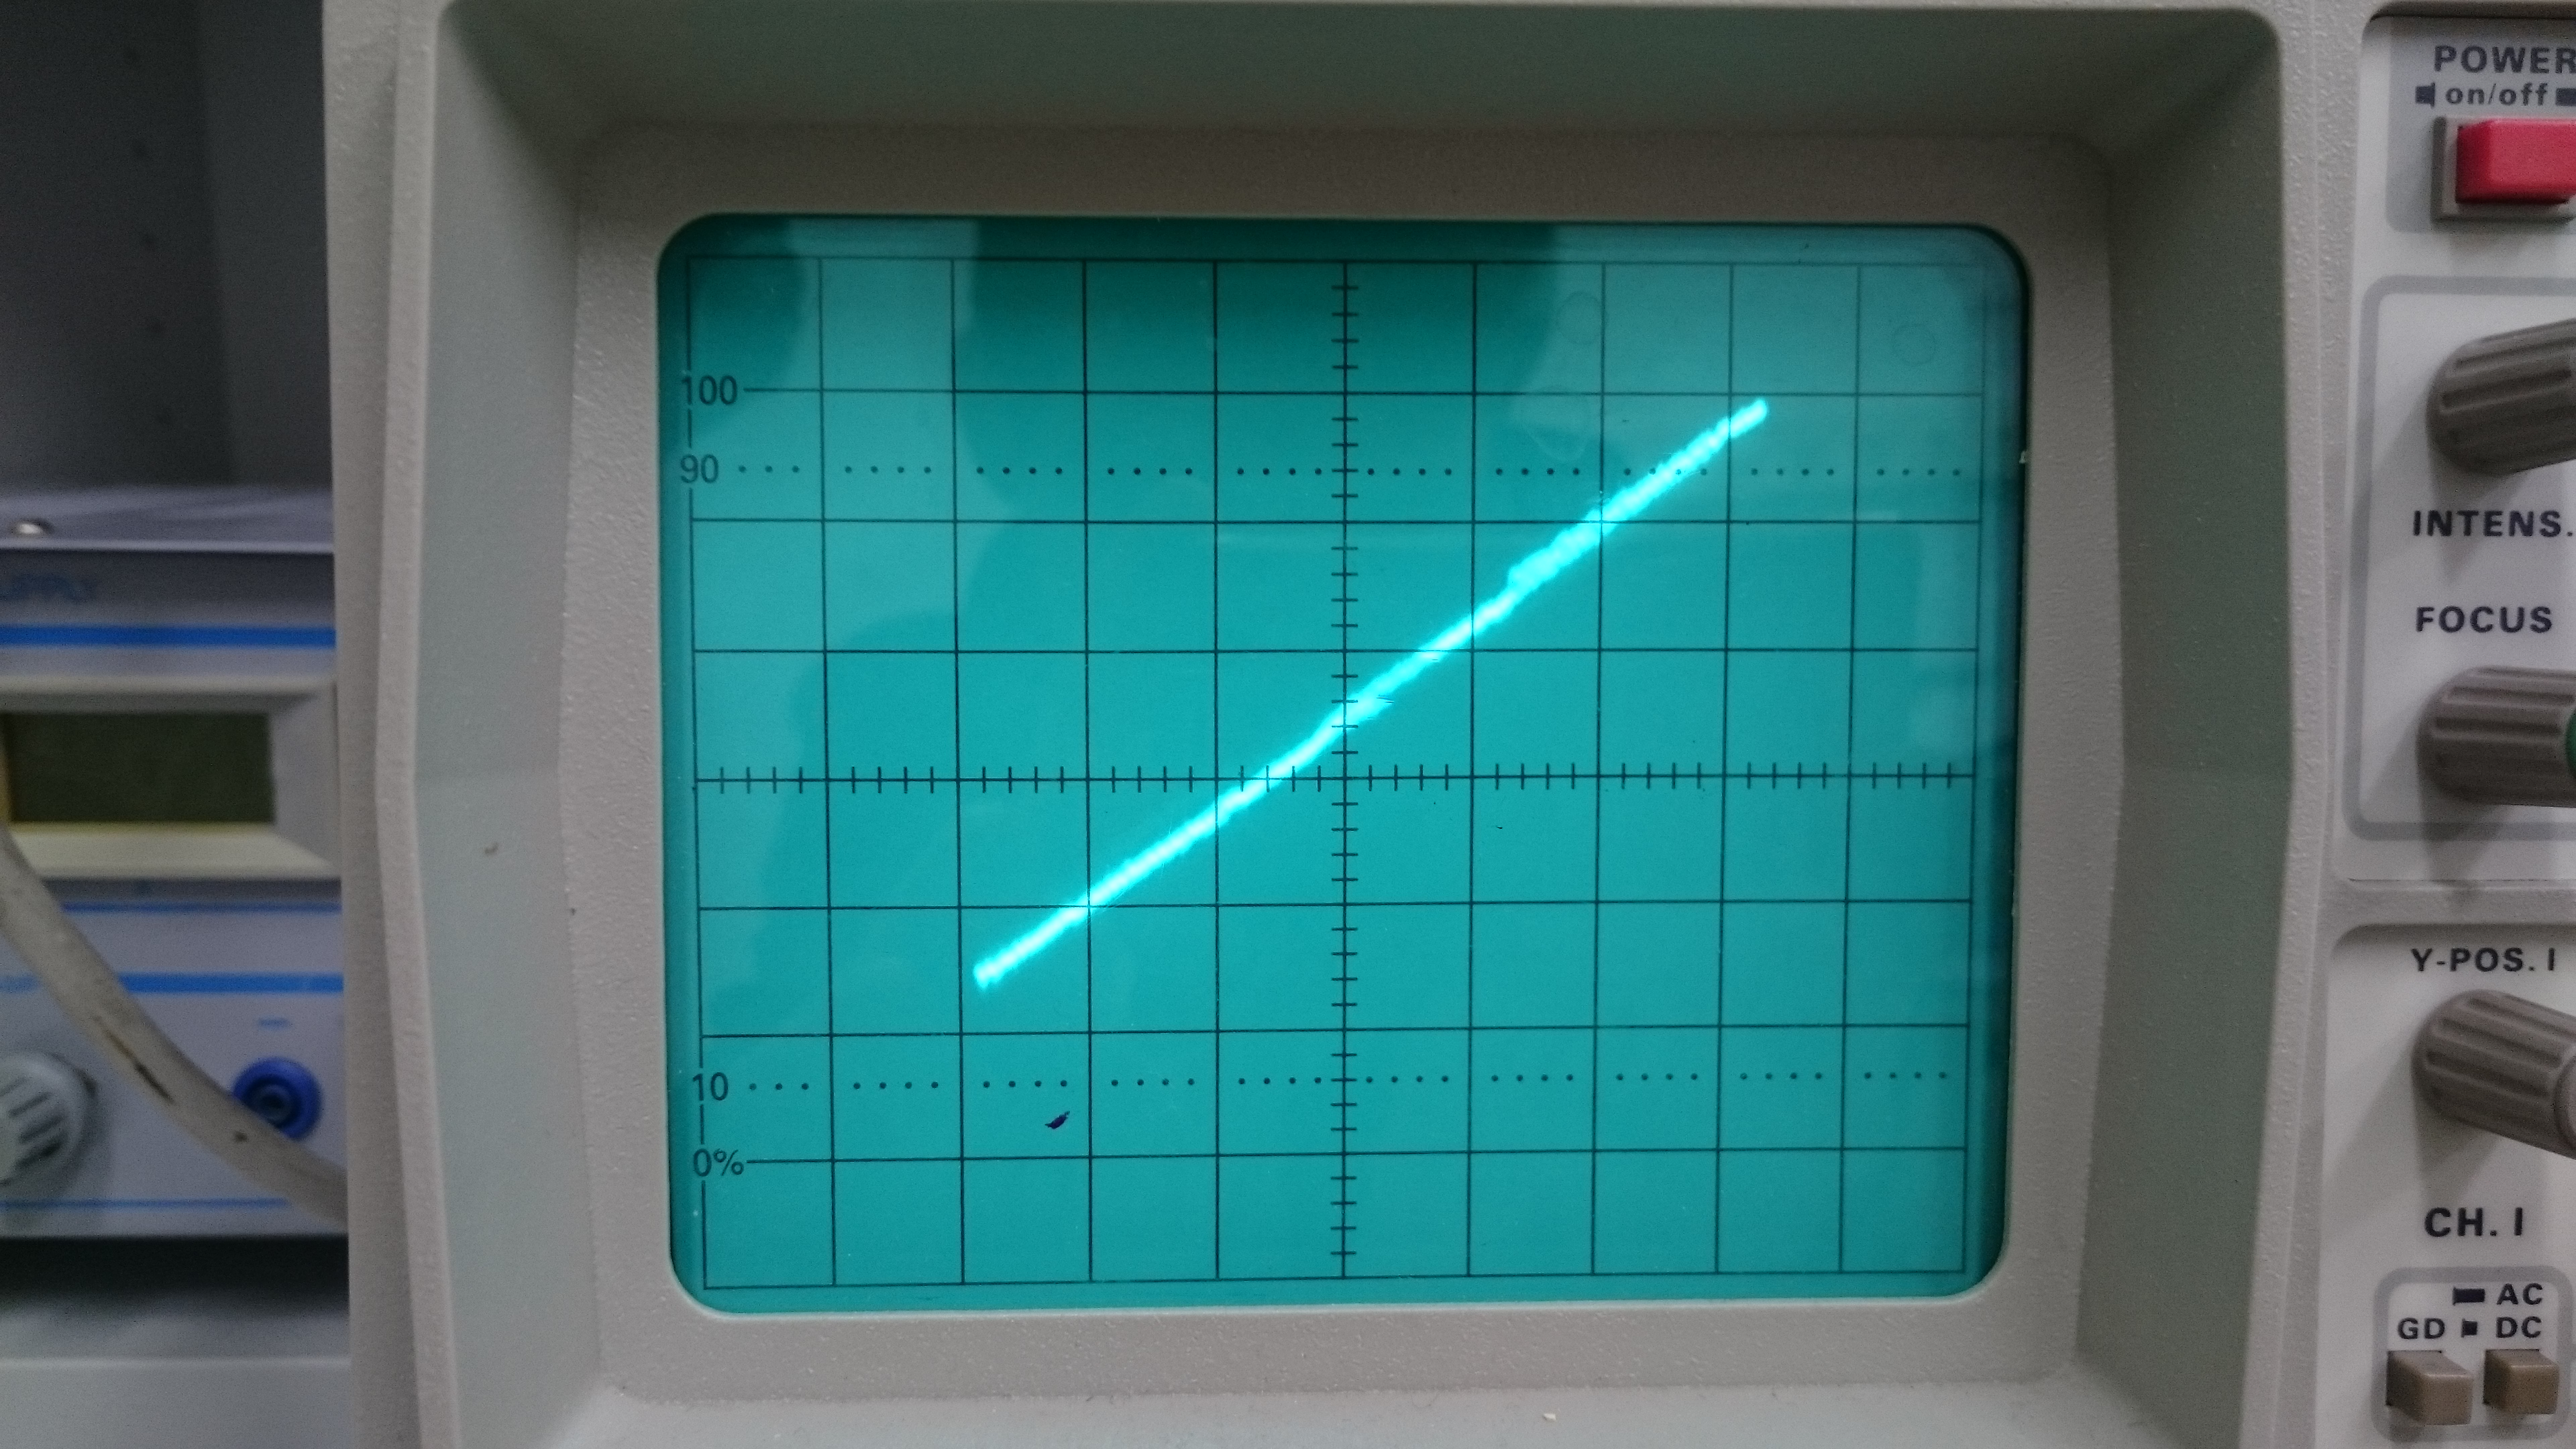
\includegraphics[scale=0.08]{messwerte/DSC_0622.JPG}
			\caption{Tantalspannung über Strom bei größerem Betrag des Wechselstromes mit eingekoppelten Mikrowellen}
			\label{nichtwelle}
		\end{figure}
		Um den Effekt deutlicher darzustellen, wären wohl stabilere Kontakte und bessere Kopplungen erforderlich gewesen. 
		Auch die Leistung des Strahlers könnte erhöht werden.
		Des Weiteren bleibt zu bemerken, dass durch den sehr provisorisch erstellten Josephson-Kontakt eine Reproduzierbarkeit der Ergebnisse unmöglich war, da selbst kleinste Schwankungen und kurze Zeiträume den Kontakt und somit die Messung stark Verändern konnten.

	% subsection gleichstrom_josephson_kontakt (end)


	\subsection{SQUID-Magnetfeldmessung} % (fold)
	\label{sub:squid_magnetfeldmessung}
	
		Wie in der Durchführung beschrieben wurde der SQUID durch die Methode der gekreuzten Drähte bewerkstelligt. 
		Das Magnetfeld wurde durch zwei Helmholtz-Spulen erzeugt und mit Hilfe eines Stromteilers bestehend aus einer Dekadenreihe konnte der Strom und somit auch das Feld sehr genau eingestellt werden.
		Nach langem Suchen des richtigen Kontaktes, der richtigen Temperatur, der korrekten Ausrichtung der Spulen und vorteilhaften Anzeige des Oszilloskops, konnte eine Einstellung gefunden werden, die die erwarteten periodischen Stromminima aufwies. 
		Diese lagen bei:

		\[ 0.33\unit{A},\quad 0.6\unit{A},\quad 0.9\unit{A},\quad 1.2\unit{A},\quad 1.48\unit{A},\quad 1.8\unit{A} \]

		Daraus lässt sich eine gemittelte Periode von circa $0.3\unit{A}$ errechnen.
		Aus der Elektrodynamik ist dann bekannt, dass sich das $B$-Feld im Mittelpunkt exakt durch folgende Gleichung berechnen lässt (äquivalent zur Bestimmung des $B$-Feldes einer Leiterschleife):
		\[ B = \mu_0 IN \dfrac{R^2}{\boxb{R^2 + \curvb{\frac{l}{2}}^2}^{\frac{3}{2}}} \]
		Es ergibt sich nun mit $R=25\unit{cm}$, $l=54\unit{cm}$ und $N=40$ folgendes: 
		\[ \Delta B = 1.9\cdot 10^{-5}\unit{T} \]
		Die Fläche des betrachteten SQUIDs folgt nun aus Grundlagen durch
		\[ A = \dfrac{\Phi_0}{\Delta B} = 1.1\cdot 10^{-10}\unit{m}^2 \]
		Dies entspricht der zu erwartenden Größenordnung.

	% subsection squid_magnetfeldmessung (end)


% section messwerte_und_auswertung (end)